\section{Introduction}
% Introduction 
% <<<
The Stokes equations \eqref{unsteady_stokes}, which are solved for an incompressible Navier-Stokes flow,
assume the Reynolds number is $Re \ll 1$ and thus convective processes are neglible in comparison to viscous processes.
We will begin with the steady-state form \eqref{steady_stokes}.
Due to this simplification, the Steady stokes equations \eqref{steady_stokes}, repeated here:
\begin{align*}
    -\mu\Delta u + \nabla p = \rho g, \quad \nabla\cdot u = 0,
\end{align*}
form a constrained linear equation. As we saw in section \ref{pressure_derivation}, the pressure term $p$ is a Lagrange multiplier introduced
with the constraint $\nabla\cdot u = 0$.
\subsection{The lid-driven cavity flow problem}
A standard test case in computational fluid dynamics is the \textit{lid-driven cavity flow} problem.
We let the domain be is $\Omega = [-1,1]^2$ and define a Dirichlet boundary condition:
\begin{equation}\label{lid_driven_boundary_condition}
    \left.u\right|_\Gamma = u_\Gamma(x,y) =
    \left\{\begin{array}{lr}
        \left(1, 0\right)^T &\text{if $y = 1$,}\\
        \left(0, 0\right)^T &\text{otherwise}.\\
        \end{array}\right.
\end{equation}
We will use a finite element method to solve the steady Stokes flow \eqref{steady_stokes} with this domain and boundary condition. A highly viscous incompressible
fluid under these conditions will form a single stable vortex.

\subsection{Attempting solution by an iterative pressure update}
% <<<
Since the steady Stokes equations are a linearly constrained vector Poisson equation,
it would be convenient to use a solution method which trivially extends our already-implemented Poisson solver.
One idea is to define a coupled system of equations replacing the constrained equation \eqref{steady_stokes}, resulting in an initial boundary value problem
in auxilliary parameter $\gamma$:
\begin{equation}
\begin{split}
    -\nu\Delta u &= -\nabla p_*,\\
    \Part{p_*}{\gamma} &= -C\nabla\cdot u,\\
    \text{with \quad} \left.u\right|_\Gamma &= u_\Gamma, u(\hat{x}, 0) = u_0(\hat{x}), \text{\quad and \quad} p_*(\hat{x}, 0) = 0,
\end{split}
\end{equation}
where $C > 0$ controls the speed of the divergence elimination.
With explicit Euler in the parameter $\gamma$, the resulting iterative fixed point method is
\begin{equation}
\begin{split}
    u^{(0)} &\leftarrow u_0,\\
    p_*^{(0)} &\leftarrow 0,\\
    -\nu\Delta u^{(n)} &\leftarrow -\nabla p_*^{(n)},\\
    p_*^{(n+1)} &\leftarrow p_*^{(n)} - \Delta\gamma C\nabla\cdot u^{(n)},
\end{split}
\end{equation}
This has some problems, notably, that if $\nabla\cdot u$ is constant the pressure gradient will remain unchanged, meaning
that $u^{(n)}$ will reach a fixed point while the pressure blows up. It is feasible that this iteration could be modified such that the only
effective fixed points occur when $\nabla\cdot u = 0$, but luckily, the method converges for the lid-driven cavity problem.

\subsubsection{Implementing the pressure iteration}
To implement this iteration, the divergence $\nabla\cdot u^{(n)}$ must be projected onto the pressure space P1.
For each pressure basis function $\psi^p_1,\cdots,\psi^p_{n_p}$, an integral is computed and stored in a vector of values
$$
    \hat{v}_{\text{proj}} \leftarrow \left[\int_\Omega \psi^p_j \nabla\cdot u^{(n)}\right]_{j=1,\cdots,n_p}.
$$
This is the $L^2$ projection of $\nabla\cdot u^{(n)}$ onto the P1 finite element space, so to retrieve the hat function coefficients,
form the P1 (Gramian) projection matrix
$$
    A \leftarrow \left[ \int_\Omega \phi^p_i\psi^p_j \right]_{i,j=1,\cdots,n_p}
$$
and solve the linear system
$$
    A\hat{v} = \hat{v}_{\text{proj}}.
$$
Due to the extreme sparsity and near-orthogonality of this system, it can be solved very efficiently. Finally,
the pressure update is
$$
    \hat{p}_*^{(n+1)} \leftarrow \hat{p}_*^{(n)} - \Delta t C \hat{v},
$$
where $\hat{p}_*^{(n)}$ denotes the vector of coefficients of hat functions which combine to $p_*^{(n)}$.
The results for the lid-driven cavity problem are displayed in figure \ref{stokes_lid_driven_weakly_incomprssible}.

\begin{figure}[H]
    \centering
    \centerline{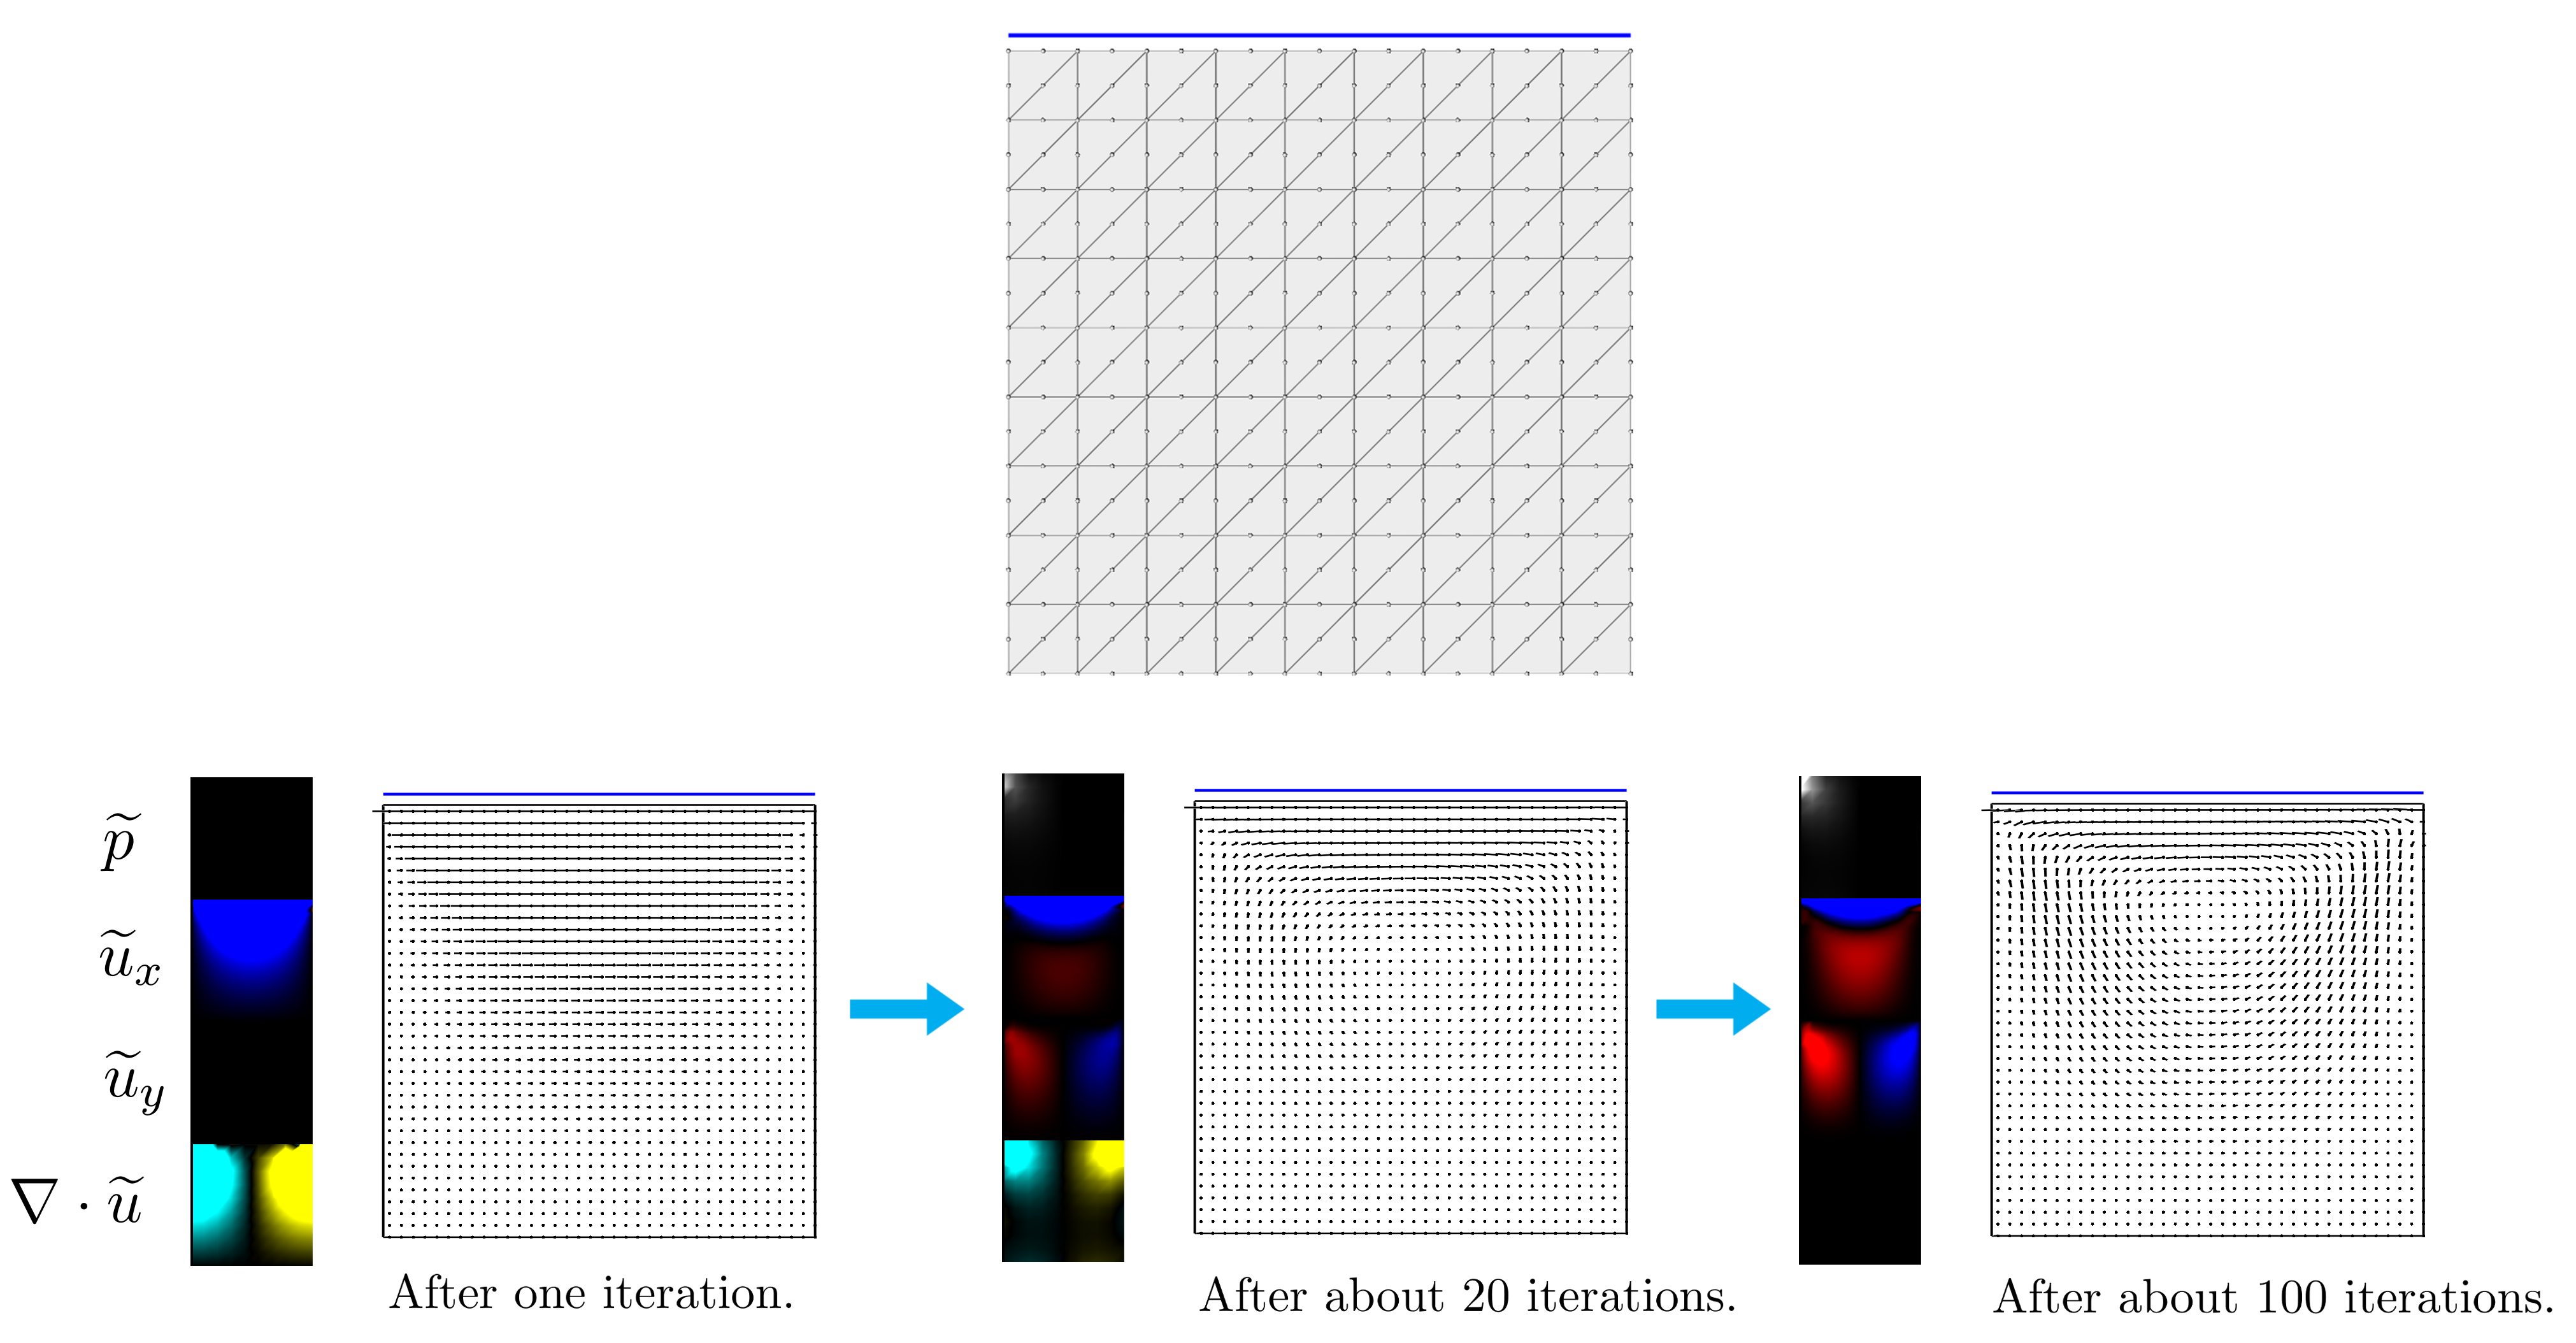
\includegraphics[width=1.3\textwidth]{figures/stokes/lid_driven_weakly_incompressible/figure.png}}
    \label{stokes_lid_driven_weakly_incomprssible}
\end{figure}
This has taken quite a large number of iterations, each iteration solving two large sparse linear systems (the Gramian system being the cheaper to solve).
However, the result is as expected, and this method is easy to implement given an already-working quadratic-element Poisson solver.

\subsection{A mixed finite element method}

As described in section \ref{pressure_derivation}, the pressure $p$ is a Lagrange multiplier that appears
when solving the optimization problem \eqref{stokes_flow_optimization}:
\begin{equation*}
\begin{aligned}
& \underset{u}{\text{minimize}}
& & E(u) =  \frac{\mu}{2} \inner{\nabla u, \nabla u} - \inner{u, \rho g}\\
& \text{subject to}
& & \nabla\cdot u = 0.
\end{aligned}
\end{equation*}

% We will begin by discretizing the \textit{unconstrained} steady Stokes equations,
% which are a vector Poisson equation:
% \begin{equation}\label{steady_stokes_unconstrained}
%     -\mu\Delta u = \rho g.
% \end{equation}
% % >>>
% \subsection{Discretizing the vector Poisson equation}\label{discretizing_vector_poisson}
% % <<<
% In principle we should keep the Stokes equation
% in integral form (using the conservative-form Cauchy momentum equation \eqref{cauchy_continuity_eulerian}), and continue as we did
% in section \ref{trial_function}. However,
% we will take a formal step to skip the reasoning of section \ref{trial_function}, typical of finite element method derivations.
% As we start with the \textit{differential} equation \eqref{steady_stokes_unconstrained}, we can introduce a trial space $\Psi$ and then ``weaken''
% the equation by integrating against $v \in \Psi$, and removing the Laplacian by integration by parts:
% \begin{equation}\label{steady_stokes_unconstrained_weak}
%     \int_\Omega -\mu\Delta u\cdot v\,dx = \int_\Omega \rho g\cdot v\,dx
%     \quad\equiv\quad
%     \int_\Omega -\mu\nabla u : \nabla v\,dx = \int_\Omega \rho g\cdot v\,dx.
% \end{equation}

% Noting that the left-hand-side of \eqref{steady_stokes_unconstrained_weak} is a bilinear form in $u$ and $v$, and the right-hand-side
% is a linear functional in $\psi$, it is standard practice (ref) to write this kind of equation as
% \begin{equation}
%     a(u, v) = f(v).
% \end{equation}
% Our subsequent derivations are much the same as in \ref{discretizing_poisson}, simplified by our new notation.
% We can now approximate $u$ in the test space $\Phi$ as $\hat{u} = \sum_{i=1}^nu_i\phi_i$. By linearity we only need to compute
% trials over the basis trial functions $\psi_j$.
% We then have the linear system of equations
% \begin{equation}\label{elliptic_bilinear_form}
%     \sum_{i=1}^n u_i a\left(\phi_i, \psi_j\right) = f(\psi_j),\quad j=1,\cdots,n,
% \end{equation}
% which can be written in matrix form as
% \begin{equation}\label{elliptic_bilinear_form_matrix}
%     A\hat{u} = \begin{bmatrix}
%             a(\phi_1, \psi_1) & \cdots & a(\phi_1, \psi_n) \\
%             \vdots & & \vdots \\
%             a(\phi_n, \psi_1) & \cdots & a(\phi_n, \psi_n)
%             \end{bmatrix}
%     \begin{bmatrix} u_1 \\ u_2 \\ \vdots \\ u_{n-1} \\ u_n \end{bmatrix}
%     =
%     \begin{bmatrix} f(\psi_1) \\ f(\psi_2) \\ \vdots \\ f(\psi_{n-1}) \\ f(\psi_{n}) \end{bmatrix}
%     = \hat{f}.
% \end{equation}
% % The matrix $A$ is symmetric positive-definite, and we can therefore think of a solution to \eqref{elliptic_bilinear_form_matrix}
% % as as a minimizer of the scalar quadratic form
% % \begin{equation}\label{elliptic_quadratic_form}
% %     \hat{E}(\hat{u}) \coloneqq \frac{1}{2} \inner{\hat{u}, A\hat{u}} - \inner{\hat{u}, \hat{f}}.
% % \end{equation}
% % This is simply a discrete realisation of the fact that we can, as described in section \ref{pressure_derivation}, think
% % of a solution to the vector Poisson equation as a minimizer of the Dirichlet energy \eqref{steady_stokes_dirichlet_energy},
% % \begin{align*}
% %     E(u) \coloneqq \int_{\Omega} \frac{\mu}{2} \inner{\nabla u, \nabla u} - \rho g\cdot u \,dx.
% % \end{align*}
% We can solve \eqref{elliptic_bilinear_form_matrix} to get a velocity field $\sum_{i=1}^n u_i\phi_i$, although in general this will not satisfy $\nabla\cdot u = 0$.
% As some preliminary analysis, if $\Phi = \Psi$ and have the same basis functions, we have a symmetric-positive-definite system. This form of linear system is known to be stably solvable,
% for example by the conjugate gradient method.
% >>>


\subsection{The weak form of the steady Stokes equations}
% <<<
As described in section \ref{pressure_derivation}, the pressure $p$ is a Lagrange multiplier that appears
when solving the optimization problem \eqref{stokes_flow_optimization}:
\begin{equation*}
\begin{aligned}
& \underset{u}{\text{minimize}}
& & E(u) =  \frac{\mu}{2} \inner{\nabla u, \nabla u} - \inner{u, \rho g}\\
& \text{subject to}
& & \nabla\cdot u = 0.
\end{aligned}
\end{equation*}

\newcommand{\trialconstraint}{{\Psi_{\text{constraint}}}}
\newcommand{\testpressure}{{\Phi_{\text{pressure}}}}
As a first idea, we can introduce $p$ as a variable to solve for. Solving for the pressure (the ``dual variable'') simultaneously with the velocity
(the ``primal variable'')
is called a primal-dual method for the optimization \eqref{stokes_flow_optimization}, and the resulting finite element method is called \textit{mixed}.
Pressure then needs to be discretized, so we introduce another test space $\testpressure$.
To get a weak form of the steady Stokes equations \eqref{steady_stokes}, which are two equations including the constraint $\nabla\cdot u = 0$, we introduce
another trial space $\trialconstraint$, whose functions will be integrated against $\nabla\cdot u$. The weak form is then
\begin{equation*}
\begin{split}
    &\int_\om \left(-\mu\Delta u + \nabla p\right)\psi\,dx = \int_\Omega \rho g\cdot\psi\,dx,\\
    &\int_\om \left(\nabla\cdot u\right) q\,dx = 0, \quad\text{where $\psi \in \Psi, q \in \trialconstraint$},
\end{split}
\end{equation*}
which by integration by parts can be written as
\begin{equation}\label{steady_stokes_weak}
\begin{split}
    &\int_\om \mu\nabla u : \nabla \psi - p\nabla\cdot \psi\,dx = \int_\om \rho g\cdot \psi\,dx,\\
    &\int_\om -\left(\nabla\cdot u\right)q\,dx = 0, \quad\text{where $\psi \in \Psi, q \in \trialconstraint$}.
\end{split}
\end{equation}
% We will be using a Bubnov--Galerkin method, so $\Psi = \Phi$ and $\Psi_{\text{constraint}} = \Phi_{\text{constraint}}$.
To simplify notation, we can introduce the ``mixed spaces''
\begin{align*}
    \Phi^\mathcal{M} = \Phi \times \Phi_{\text{constraint}}
    \text{\quad and \quad}
    \Psi^\mathcal{M} = \Psi \times \Psi_{\text{constraint}}
\end{align*}
and, using the notation of \cite{taylor_hood_fenics}, \eqref{steady_stokes_weak} can be rewritten as
\begin{equation}\label{steady_stokes_bilinear_form}
    a((u, p), (\psi, q)) = L((v, q)), \quad\quad (u,p) \in \Phi^\mathcal{M},\quad (\psi, q) \in \Psi^\mathcal{M}
\end{equation}
where $a$ is a bilinear form defined by
\begin{align*}
    a((u, p), (\psi, q)) = \int_\Omega \nabla u : \nabla\psi - p\nabla\cdot \psi - \left(\nabla\cdot u\right)q\,dx
\end{align*}
and $f$ is a linear functional defined by
\begin{align*}
    L((v, q)) = \int_\Omega \rho g\cdot\psi\,dx.
\end{align*}

---todo: Use $H^1$, $L^2$, discretize spaces later.
\subsection{Taylor-Hood mixed finite elements for the Stokes problem}

In the derivations of chapter (), many of the manipulations were trivial applications of linearity and splitting of
boundary and interior terms, and is standard in the finite element literature to define forms such as the $a$ and $L$ above.
If we discretize to $n$ (interior) basis functions
there are $2n$ basis functions for the mixed test and trial spaces, which are the natural choice:
\begin{equation}\label{mixed_space_basis_functions}
\begin{split}
    \Phi^\mathcal{M} &= \text{span}\left(
        (\phi_1, 0),\cdots,(\phi_n, 0), (0,\phi_1^p),\cdots,(0,\phi_n^p)
    \right),\\
    \Psi^\mathcal{M} &= \text{span}\left(
        (\psi_1, 0),\cdots,(\psi_n, 0), (0,\psi_1^p),\cdots,(0,\psi_n^p).
    \right)
\end{split}
\end{equation}


All we must do is plug approximations, from finite dimensional function spaces, into the weak form \eqref{steady_stokes_bilinear_form}, 
while performing trial integrals only over the basis functions in the a finite dimensional mixed trial space, resulting in the
linear system of equations
\begin{equation}\label{stokes_flow_mixed_equations_1}
\begin{split}
    a((\tilde{u}, \tilde{p}), (\psi_j, 0)) &= L((\psi_j, 0)), \quad j = 1,\cdots,n\\
    a((\tilde{u}, \tilde{p}), (0, \psi^p_j)) &= L((0, \psi^p_j)), \quad j = 1,\cdots,n,
\end{split}
\end{equation}
We must choose the finite-dimensional spaces $\Phi,\Psi,\Phi_{\text{constraint}},$ and $\Psi_{\text{constraint}}$.
The algorithm for the Stokes problem, with Dirichlet boundary conditions, will then consist of forming the matrix and right-hand side of
\eqref{stokes_flow_abstract_linear_system}, then passing it to a linear solver.

We will use the Bubnov--Galerkin method (letting $\Psi = \Phi$), and make a standard choice of mixed finite element space,
    $$\Phi^\mathcal{M} = \Phi \times \Phi_{\text{constraint}} = P^2_2 \times P^1,$$
where $P_2$ and $P_1$ denote, respectively, the piecewise quadratic and piecewise linear elements derived in chapter ().
This mixed space is formed from the ``Taylor-Hood elements'', and is known to result in a stable method for the Stokes problem\footnote{
While we could choose just about any spaces for the non-mixed method for the Poisson problem, which is elliptic, the Stokes flow problem
inherently involves a Lagrange multiplier, and is known as a ``saddle point problem''. The resulting finite element matrix is hyperbolic.
The Taylor-Hood elements satisfy the Ladyzhenskaya--Babu\v ska--Brezzi (LBB) condition, which
is a theoretical result which guarantees that the resulting linear system for the Stokes problem will be well-conditioned.
If we took $P^1 \times P^1$ instead, for example, this condition would not hold.
}.

So we don't have to repeat the equations for each kind of mixed trial function, as we do in \eqref{stokes_flow_mixed_equations_1}, we can use the mixed basis order \eqref{mixed_space_basis_functions} and define $\phi^\mathcal{M}_l$ to be the $l$'th mixed basis
function in this order (e.g. $\psi^\mathcal{M}_1 = (\psi_1, 0)$ and $\psi^\mathcal{M}_{n+1} = (0, \psi^p_1)$).

\begin{aside}
\textit{A note on tensor notation for the vector field space}
\vskip 0.1in

The space $P^2_2$ here is a space of piecewise quadratic vector fields formed as $P^2_2 = P^2 \times P^2$.
This represents the velocity field by two functions in the usual scalar quadratic space $P^2$.
This is the simplest way to construct a finite element space of vector fields, although others (not based on a product construction) are possible.
We define $\partial x$ and $\partial y$ to be the unit vector fields on the domain $\Omega$.
The basis functions for $P^2_2$ are the natural choice of vector fields $\phi^\text{scalar}_1\partial x$, $\phi^\text{scalar}_1\partial y$, $\cdots$, $\phi^\text{scalar}_n\partial x$, $\phi^\text{scalar}_n\partial y$.
However, we would like to think of the velocity coefficients as vector samples, rather than scalar coefficients
of this array of $2n$ basis vector fields. We can do this by letting $\phi_1,\cdots,\phi_n$ be aggregates of axis-aligned vector fields:
    $$
        \phi_i = \begin{bmatrix}
        \phi_{ix} \coloneqq \phi^\text{scalar}_{i}\partial x\\
        \phi_{iy} \coloneqq \phi^\text{scalar}_{i}\partial y\end{bmatrix}.
    $$
We can then represent the interior variation as
    $$\tilde{u}_\text{interior} = \sum_{i=1}^n u_i \cdot \phi_i.$$
It is important to keep this in mind, as although this notation is natural, it may cause confusion:
While $a$ is a bilinear form, the value $a((\phi_1, 0), \psi^\mathcal{M}_4)$, for example, is actually ``vectorized''
into
    $$
        \begin{bmatrix}
            a((\phi_{1x}, 0), \psi^\mathcal{M}_4)\\
            a((\phi_{1y}, 0), \psi^\mathcal{M}_4)
        \end{bmatrix}.
    $$
This is contracted with the vector coefficient $u^1$ to get a scalar:
    $$
        u^1 \cdot a((\phi_1, 0), \psi^\mathcal{M}_4)
    = u^1_x a((\phi_{1x},0), \psi^\mathcal{M}_4)
        + u^1_y a((\phi_{1y},0), \psi^\mathcal{M}_4).
    $$
\end{aside}

As in chapter (), we let $u$ be approximated by
    $$\tilde{u} = \tilde{u}_\Gamma + \tilde{u}_\text{interior} = \tilde{u}_\Gamma + \sum_{i=1}^n u_i\cdot \phi_i,$$
where $\tilde{u}_\Gamma \in \Phi^*$ approximates the Dirichlet boundary function $\left.u\right|_\Gamma = u_\Gamma$,
and $\tilde{u}_{\text{interior}} \in \Phi$ is the ``interior variation''. A boundary condition for pressure is not given
(---todo: Should the pressure have a Dirichlet boundary set to $0$?)
    $$\tilde{p} = \sum_{i=1}^n p_i\phi^p_i.$$

Now \eqref{stokes_flow_mixed_equations_1} expands to,
rearranging constants to the right-hand side,
\begin{equation}\label{stokes_flow_abstract_linear_system}
\begin{split}
    \sum_{i=1}^n u_i\cdot a((\phi_i, 0), \psi^\mathcal{M}_l) + \sum_{i=1}^n p_ia((0, \phi_i^p), \psi^\mathcal{M}_l)
        = L(\psi^\mathcal{M}_l) - a((\tilde{u}_\Gamma, 0), \psi^\mathcal{M}_l),\\
    l = 1,\cdots,2n.
\end{split}
\end{equation}
As explained in the note on tensor notation, the left-most summation is over contractions of $u^i$ with the ``vectorized''
bilinear form $a$, as $\phi_i$ is an aggregate of vector fields, $\phi_i = (\phi_{ix}, \phi_{iy})^T$.

The $\psi_l^\mathcal{M}$ mixed trial function ranges over all basis trial functions, \ref{mixed_space_basis_functions}.
Suppose $\psi_l^\mathcal{M} = (\psi_1, 0)$. We have $\psi_1 = \phi_1$ (due to using Bubnov--Galerkin), which is the aggregate of vector fields defined in the note on tensor notation. Therefore this one apparent equation, with $\psi_l^\mathcal{M} = (\psi_1, 0)$ actually defines two equations,
\begin{align*}
    \sum_{i=1}^n u_i\cdot a((\phi_i, 0), (\psi_{1x}, 0)) + \sum_{i=1}^n p_ia((0, \phi_i^p), (\psi_{1x}))
        = L((\psi_{1x}, 0)) - a((\tilde{u}_\Gamma, 0), (\psi_{1x}, 0)),\\
    \sum_{i=1}^n u_i\cdot a((\phi_i, 0), (\psi_{1y}, 0)) + \sum_{i=1}^n p_ia((0, \phi_i^p), (\psi_{1y}))
        = L((\psi_{1y}, 0)) - a((\tilde{u}_\Gamma, 0), (\psi_{1y}, 0)).
\end{align*}

Therefore equation \eqref{stokes_flow_abstract_linear_system}
forms a $(2n + n_p) \times (2n + n_p)$ linear system (with $2n$ coefficients for the velocity, $n_p$ for the pressure).

\begin{aside}
\textit{Automation}
\vskip 0.1in

It has been very beneficial to go from the weak form of our specific Stokes problem
\eqref{steady_stokes_weak} to the abstract form \eqref{steady_stokes_bilinear_form} in terms of the forms $a$ and $L$.
When the approximating solutions $\tilde{u}$ and $\tilde{p}$ are plugged in, all that
takes place is a linear expansion and rearrangement, accounting for boundary terms.

It is feasible that this process could be automated, as in, we could pass a symbolic representation of the weak form
\eqref{steady_stokes_weak}, a mesh discretizing the domain, a specification of the finite element function spaces
(in some symbolic notation such as ``\texttt{P1 x P2\_2}''),
and boundary conditions. This is all the data specific to our problem --- with this data, the finite element algorithm
is fully specified, and it is a routine task to do all the expansions and rearrangements to specify the linear system,
then to write a matrix assembly algorithm to traverse the mesh and construct this system.

This in fact has been done
\cite{fenics_book} \cite{DOLFIN} \cite{firedrake} \cite{automating_fem},
and is an active area of research.

\end{aside}




% The approximated pressure is $\tilde{p} \in \Phi_{\text{pressure}}$ where
%     $$\Phi_{\text{pressure}} = \text{span}(\phi_{pi},\cdots,\phi_{pn}).$$
% The pressure is zero on the boundary ($\left.p\right|_\Gamma = 0$), as it is only meaningful with respect to
% integrals over interior control volumes,
% so we have
%     $$\tilde{p} = \sum_{i=1}^n p_i \phi_{pi}.$$
% The velocity vector field $u$ is discretized as
%     $$\tilde{u} =  \phi_\Gamma + \phi = \phi_\Gamma + \sum_{i=1}^n u_i\phi_i$$
% where $\phi_\Gamma$ is the boundary approximation in $\Phi^*$, as in chapter ().

We simply plug these approximation definitions into the weak form \eqref{steady_stokes_weak}, resulting in the
linear system of equations:
\begin{equation}\label{steady_stokes_linear_system}
\begin{split}
&\sum_{i=1}^n \left[u_i\cdot \int_\Omega -\mu\nabla\phi_i : \nabla\psi_j\,d\hat{x}
        + p_i\int_{\Omega} -\psi_j \cdot \nabla\phi_{pi}\,d\hat{x}\right]
    = \int_\Omega \rho g\cdot\psi_j
        + \mu\nabla\phi_\Gamma :\nabla\psi_j \,d\hat{x},\\
&\sum_{i=1}^n u_i \cdot \int_\Omega -\phi_i \cdot \nabla q_j \,d\hat{x}
    = \int_\Omega \phi_\Gamma \cdot \nabla q_j \,d\hat{x},
\quad\quad j=1,\cdots,n.
\end{split}
\end{equation}

% To simplify matters, we let the vector field test and trial spaces be direct sums of scalar function spaces:
% $$
%     \Phi^* = \Phi^*_s \oplus \Phi^*_s,
%     \quad
%     \Psi^* = \Psi^*_s \oplus \Psi^*_s,
% $$
% where the $s$ subscript denotes ``scalar''. This means
% that the first equation in \eqref{steady_stokes_linear_system} splits into
% two equations, for the $x$ and $y$ components of the velocity $u$.
% Equation \eqref{steady_stokes_linear_system} is a $3n \times 3n$ linear system which (with the right choice of test and trial spaces) will be rank $3n - 1$,
% as the pressure is defined up to a constant.

% Taylor-Hood elements
% https://fenicsproject.org/olddocs/dolfin/1.5.0/python/demo/documented/stokes-taylor-hood/python/documentation.html



% We introduce notation for the bilinear and linear forms in \eqref{steady_stokes_weak}:
% \begin{equation}
% \begin{split}
%     a(u, v) &\coloneqq \int_\om-\mu\nabla u : \nabla v\,dx,\quad\text{for $u \in \Phi, v \in \Psi$},\\
%     \hat{b}(p, v) &\coloneqq \int_\om-\left(\nabla\cdot v\right)p\,dx,\quad\text{for $p \in \testpressure, v \in \Psi$},\\
%     b(u, q) &\coloneqq \int_\om-\left(\nabla\cdot u\right)q\,dx,\quad\text{for $u \in \Phi, q \in \trialconstraint$},\\
%     f(v) &\coloneqq \int_\om \rho g\cdot v\,dx\quad\text{for $v \in \Psi$}.
% \end{split}
% \end{equation}
% Although they have the same form, $b$ and $\hat{b}$ are distinguished as they take inputs in different function spaces.
% We now have a simplified notation for the weak form \eqref{steady_stokes_weak},
% \begin{equation}\label{steady_stokes_weak_notation}
% \begin{split}
%     &a(u, v) + \hat{b}(p, v) = f(v),\\
%     &b(u, q) = 0, \quad\text{where $v \in \Psi, q \in \trialconstraint$}.
% \end{split}
% \end{equation}
% % Solving for $u^*$ in the equation $a(u^*, v) = f(v)$ is the standard vector Poisson equation, resulting in a symmetric-positive-definite
% % system when the test and trials spaces are discretized. We can imagine letting $p = 0$ and solving for $u^*$.
% % The first condition of \eqref{steady_stokes_weak_notation} will hold, but the second condition (does $b(u^*, q) = 0$?) generally will not.
% Working with discrete function spaces, we get a $2n\times 2n$ linear system in the unknowns $u_1,\cdots,u_n$ and $p_1,\cdots,p_n$,
% \begin{equation}
% \begin{split}
%     &\sum_{i=1}^n u_i a\left(\phi_i, \psi_j\right) + \sum_{i=1}^np_i\hat{b}\left(\phi^C_i, \psi_j\right) = f(\psi_j),\\
%     &\sum_{i=1}^nu_ib\left(\phi_i, \psi^C_j\right) = 0,\quad j=1,\cdots.n.
% \end{split}
% \end{equation}
% To emphasize the linear system structure of \eqref{steady_stokes_weak_notation}, the block matrix form is:
% \begin{equation}\label{steady_stokes_matrix}
% \def\arraystretch{1.5}
% \begin{split}
%     M\hat{x}
%     &= \begin{bmatrix}
%             A & \hat{B} \\
%             B & 0
%     \end{bmatrix}\hat{x} \\
%     &= \left[\begin{array}{@{}ccc|ccc@{}}
%             a(\phi_1, \psi_1) & \cdots & a(\phi_1, \psi_n)     & \hat{b}(\phi^C_1, \psi_1) & \cdots & \hat{b}(\phi^C_1, \psi_n) \\
%             \vdots & & \vdots                                  & \vdots & & \vdots \\
%             a(\phi_n, \psi_1) & \cdots & a(\phi_n, \psi_n)     & \hat{b}(\phi^Cn, \psi_1) & \cdots & \hat{b}(\phi^C_n, \psi_n) \\
%             \hline
%             b(\phi_1, \psi^C_1) & \cdots & b(\phi_1, \psi^C_n) & 0 &\cdots& 0      \\
%             \vdots & & \vdots \\                               & \vdots & & \vdots \\
%             b(\phi_n, \psi^C_1) & \cdots & b(\phi_n, \psi^C_n) & 0 &\cdots& 0       
%     \end{array}\right]
%     \left[\begin{array}{c} u_1 \\ \vdots \\ u_n \\ \hline p_1 \\ \vdots \\ p_n \end{array}\right]
%     =
%     \left[\begin{array}{c} f(\psi_1) \\ \vdots \\ f(\psi_{n}) \\ \hline 0 \\ \vdots \\ 0 \end{array}\right]
%     = \hat{b}.
% \end{split}
% \end{equation}
% \subsubsection{Is this method reasonable?}
% For the vector Poisson equation, letting $\Phi = \Psi$, we ended up with a symmetric-positive-definite system \eqref{elliptic_bilinear_form_matrix}, which is known to be stably solvable.
% We can ask how reasonable it is to solve \eqref{steady_stokes_matrix}, and what trial and test spaces we should use.
% In fact, in the problem \eqref{steady_stokes_weak_notation}, and more generally in a ``saddle point problem'', arising
% in Lagrange-multiplier methods for constrained PDEs, we should not choose just any test and trial spaces.
% The Ladyzhenskaya--Babu\v{s}ka--Brezzi condition, discussed later, enforces restrictions on choices that result in a stable method.
% We will until then continue with computations.
% 
% \subsubsection{Results and visualisation}
% \vskip 0.2in
% (results and visualisation)
% \vskip 0.2in
% % >>>
% \subsection{Discretizing the unsteady Stokes equations}\label{discretizing_unsteady_stokes}
% % <<<
% \newcommand{\uprev}{{u_{\text{prev}}}}
% The steady Stokes above are the stable state of the time-dependent Stokes flow,
% after the transient flow behaviour settles down. The unsteady Stokes equations \eqref{unsteady_stokes} are
% \begin{equation*}
%     \rho\Part{u}{t} = \mu\Delta u + \rho g - \nabla p, \quad \nabla\cdot u = 0.
% \end{equation*}
% These form an initial-boundary-value problem, and this will be our first attempt at discretizing a PDE in time.
% We could think of solving with the test and trial spaces over the domain $\Omega \times [0, T)$, but this is typically not done due to the memory costs,
% and different qualitative meaning of the time variable \cite{ham_fem}. Instead, we will use an implicit-Euler finite difference in time: 
% \begin{equation}\label{unsteady_stokes_implicit_euler}
%     \frac{\rho}{\Delta t} \left(u^{(n)} - u^{(n-1)}\right) = \mu\Delta u^{(n)} + \rho g - \nabla p^{(n)}, \quad \nabla\cdot u^{(n)} = 0,
% \end{equation}
% where $\Delta t$ is a fixed time step, and $u^{(n)}$ and $p^{(n)}$ is the solution at time $t_n = n\Delta t$. We can weaken each step
% \eqref{unsteady_stokes_implicit_euler}
% by integrating against trial functions $v \in \Psi$ and $q \in \trialconstraint$, performing integration by parts as in section \ref{discretizing_steady_stokes},
% and rearranging the knowns and unknowns. We can also let $u$ be $u^{(n)}$, $p$ be $p^{(n)}$, and $\uprev$ be $u^{(n-1)}$ in the above to simplify
% subsequent notation. The weak form of \eqref{unsteady_stokes_implicit_euler} is then:
% % \begin{equation}\label{unsteady_stokes_implicit_euler_weak}
% % \begin{split}
% %     \frac{\rho}{\Delta t} \int_\om \left(u^{(n)} - u^{(n-1)}\right)\cdot v\,dx
% %         &= \int_\om \mu\nabla u^{(n)}:\nabla v + \rho g\cdot v + \left(\nabla\cdot v\right) p^{(n)}\,dx,\\
% %     \quad \int_\om \left(\nabla\cdot u^{(n)}\right) q\,dx &= 0.
% % \end{split}
% % \end{equation}
% \begin{equation}\label{unsteady_stokes_implicit_euler_weak}
% \begin{split}
%     \int_\om \frac{\rho}{\Delta t} u\cdot v - \mu\nabla u:\nabla v - \left(\nabla\cdot v\right)p\,dx
%         &= \int_\om \frac{\rho}{\Delta t}\uprev\cdot v + \rho g \cdot v\,dx,\\
%     \quad \int_\om \left(\nabla\cdot u\right) q\,dx &= 0,
% \end{split}
% \end{equation}
% % and with the linear form definitions in section \ref{discretizing_steady_stokes} this is
% % \begin{equation}\label{unsteady_stokes_implicit_euler_weak_notation}
% % \begin{split}
% %     &\int_\om \frac{\rho}{\Delta t} u\cdot v \,dx + a(u, v) + \hat{b}(p, v) = \int_\om \frac{\rho}{\Delta t} \uprev\cdot v \,dx + f(v),\\
% %     &b(u, q) = 0, \quad\text{where $v \in \Psi, q \in \trialconstraint$}.
% % \end{split}
% % \end{equation}
% We can define the linear forms as
% \begin{equation}
% \begin{split}
%     a(u, v) &\coloneqq \int_\om\frac{\rho}{\Delta t}u\cdot v -\mu\nabla u : \nabla v\,dx,\quad\text{for $u \in \Phi, v \in \Psi$},\\
%     \hat{b}(p, v) &\coloneqq \int_\om-\left(\nabla\cdot v\right)p\,dx,\quad\text{for $p \in \testpressure, v \in \Psi$},\\
%     b(u, q) &\coloneqq \int_\om-\left(\nabla\cdot u\right)q\,dx,\quad\text{for $u \in \Phi, q \in \trialconstraint$},\\
%     f(v) &\coloneqq \int_\om \frac{\rho}{\Delta t}\uprev\cdot v + g\cdot v\,dx\quad\text{for $v \in \Psi$}
% \end{split}
% \end{equation}
% to reexpress \eqref{unsteady_stokes_implicit_euler_weak} in the notation
% \begin{equation}
% \begin{split}
%     &a(u, v) + \hat{b}(p, v) = f(v),\\
%     &b(u, q) = 0, \quad\text{where $v \in \Psi, q \in \trialconstraint$}.
% \end{split}
% \end{equation}
% This is the same structure as in the steady Stokes system \eqref{steady_stokes_weak_notation},
% and so the matrix block structure is the same as in \eqref{steady_stokes_matrix}. Therefore, every step we need to solve a linear system
% that is very similar to the steady Stokes problem. In fact this step can be thought of as successively introducing the momentum source $\rho g$
% (ignoring convection), while solving for the updated pressure needed to keep the fluid non-compressed.
% 
% \subsubsection{Discretizing the initial condition}
% We may have some analytically determined, or otherwise, initial velocity field $u$ with $\nabla\cdot u = 0$.
% We would like to form $u^{(0)}$ in order to start the iteration. The velocity $u$ should be projected in some way into the test space $\Psi$.
% Enforcing $u^{(0)}$ to give the same ``blurred average'' value when evaluated against a trial function,
% \begin{equation}\label{initial_velocity_projection}
%     \int_\om u^{(0)}\cdot v\,dx = \int_\om u \cdot v\,dx,\quad \forall v \in \Psi,
% \end{equation}
% gives a linear system
% \begin{equation}\label{initial_velocity_projection_linear_system}
%     \sum_{i=1}^n u^{(0)}_i \int_\om \phi_i \cdot \psi_j\,dx = \int_\om u\cdot \psi_j\,dx,
%     \quad j=1,\cdots,n.
% \end{equation}
% Solving this linear system for the $u^{(0)}_i$ gives $u^{(0)} = \sum_{i=1}^n u^{(0)}_i \phi_i$ as a projection of $u$ onto $\Phi$.
% This projection is orthogonal if $\Phi = \Psi$, and therefore could be considered the ``best'' such projection in the Euclidean norm.
% This is the standard Gramian matrix construction for projection in approximation theory \cite{approximation_theory}.
% 
% % >>>
% >>>
% 
% \section{Solving non-linear equations}
% % <<<
% \subsection{A non-linear Poisson equation}
% \subsection{A non-linear heat equation}
% \subsection{The Burgers equation}
% % >>>
% 
% \section{Implementing finite element methods}
% % <<<
% \subsection{The Ciarlet definition of a finite element space}
% \cite{ciarlet}, \cite{ham_fem}, \cite{fenics_book}
% 
% 
% % Discuss Ciarlet definition, difference between FEM, spectral etc. FEM uses a domain partition to help in constructing the basis functions.
% 
% One great utility of the finite element method is that it is compatible with complex geometric domains and domain partitions.
% Some greater effort is needed to apply finite differences correctly across complex boundaries, and it is non-trivial to implement
% a varying resolution of the discretisation. In the finite element method, however, specifying the test and trial functions over
% a square grid is much the same as specifying them over, for example, a surface mesh of arbitrary topology. For modelling, for example,
% heat transfer in a complex solid, one can construct basis functions over a grid on the interior, and over cut-off boundary cells near the exterior.
% This is all in principle, of course, as one needs to
% \begin{enumerate}
%     \item Break the domain up into small pieces.
%     \item Construct the basis and trial functions over this domain partition (e.g. by finding polynomial coefficients).
%     \item Compute all inner products of test and trial functions, and their relevant derivatives, either numerically or analytically.
%     \item Solve possibly many huge sparse linear systems, while possibly changing the structure of the domain partition (requiring changes to the inner products).
% \end{enumerate}
% 
% Step (1) is already a field in itself, as evidenced by the open source tool TetGen \cite{tetgen}.
% TetGen is a small tool whose primary purpose is to perform \textit{constrained Delaunay tetrahedralization}, given a solid boundary and a point cloud on the interior.
% This constructs a valid tetrahedral partition intended for finite element solvers. The partition is efficiently created in a very robust manner in over 36k lines of C code. TetGen is part of the geometric backbone of many FEA tools (references).
% % >>>


% \begin{figure}[H]
%     \centering
%     \centerline{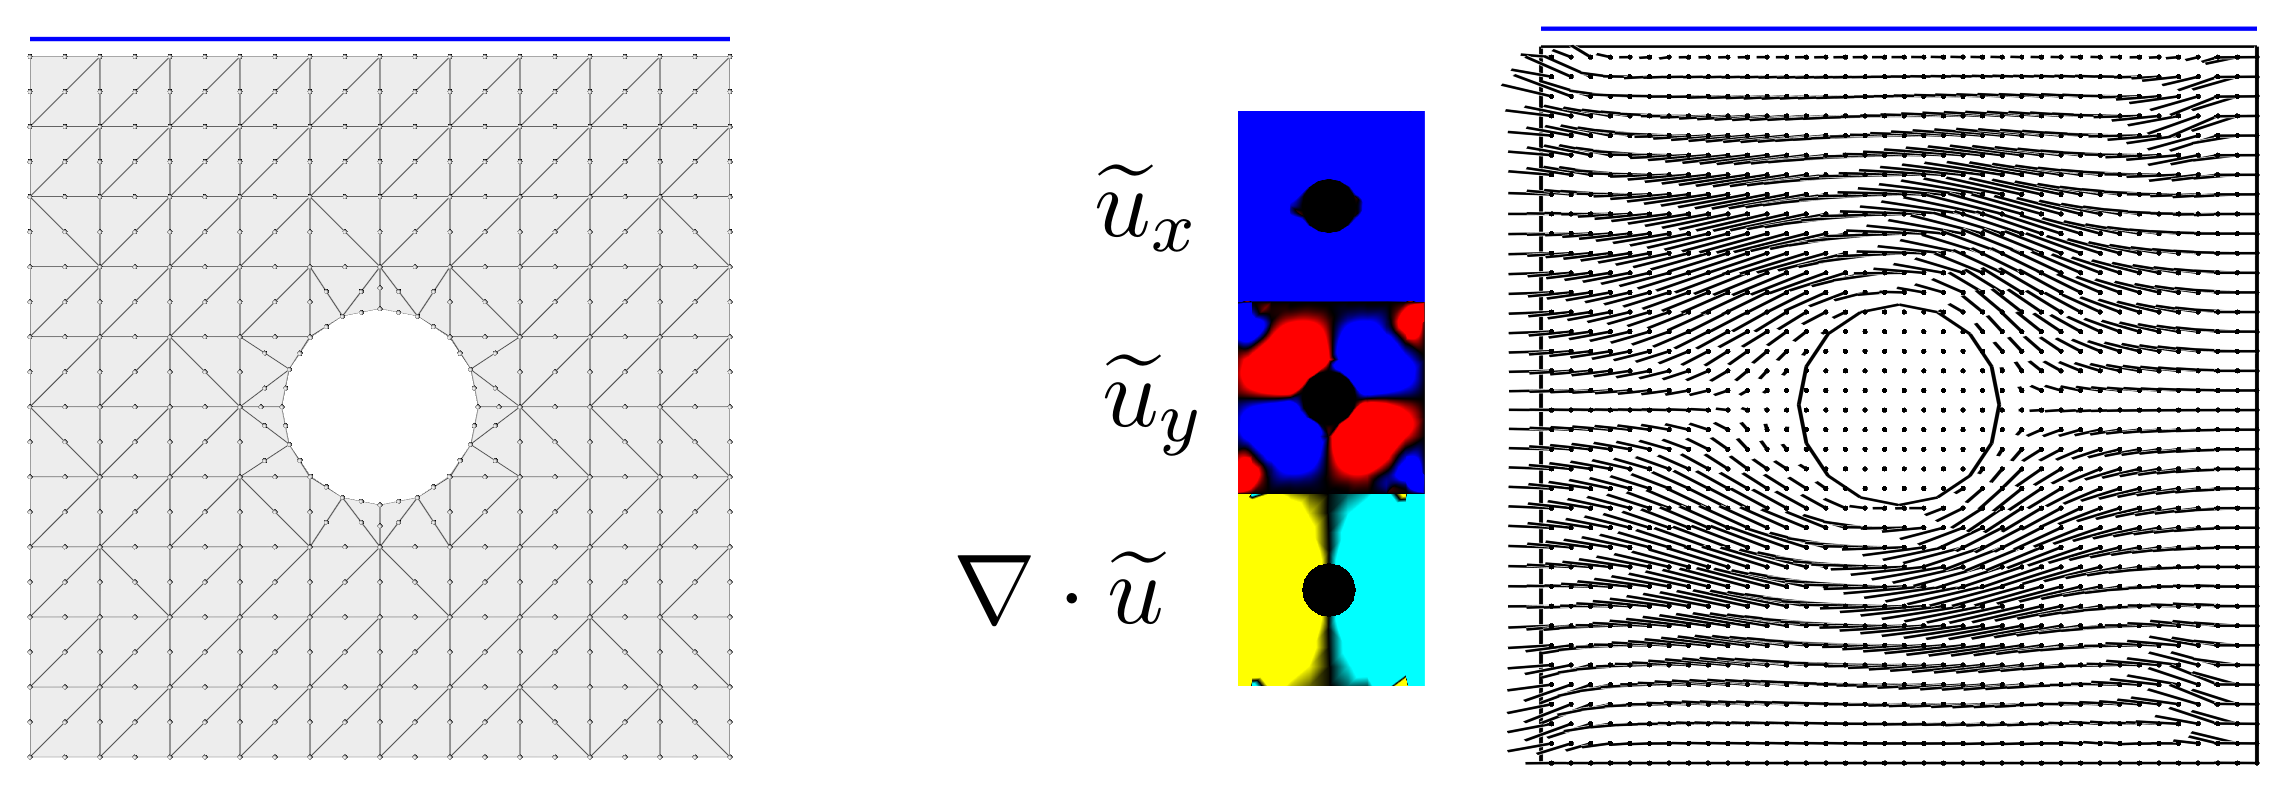
\includegraphics[width=0.8\textwidth]{figures/stokes/obstruction_failed_weakly_incompressible/figure.png}}
%     \label{stokes_obstruction_failed_weakly_incompressible}
% \end{figure}

\begin{figure}[H]
    \centering
    \centerline{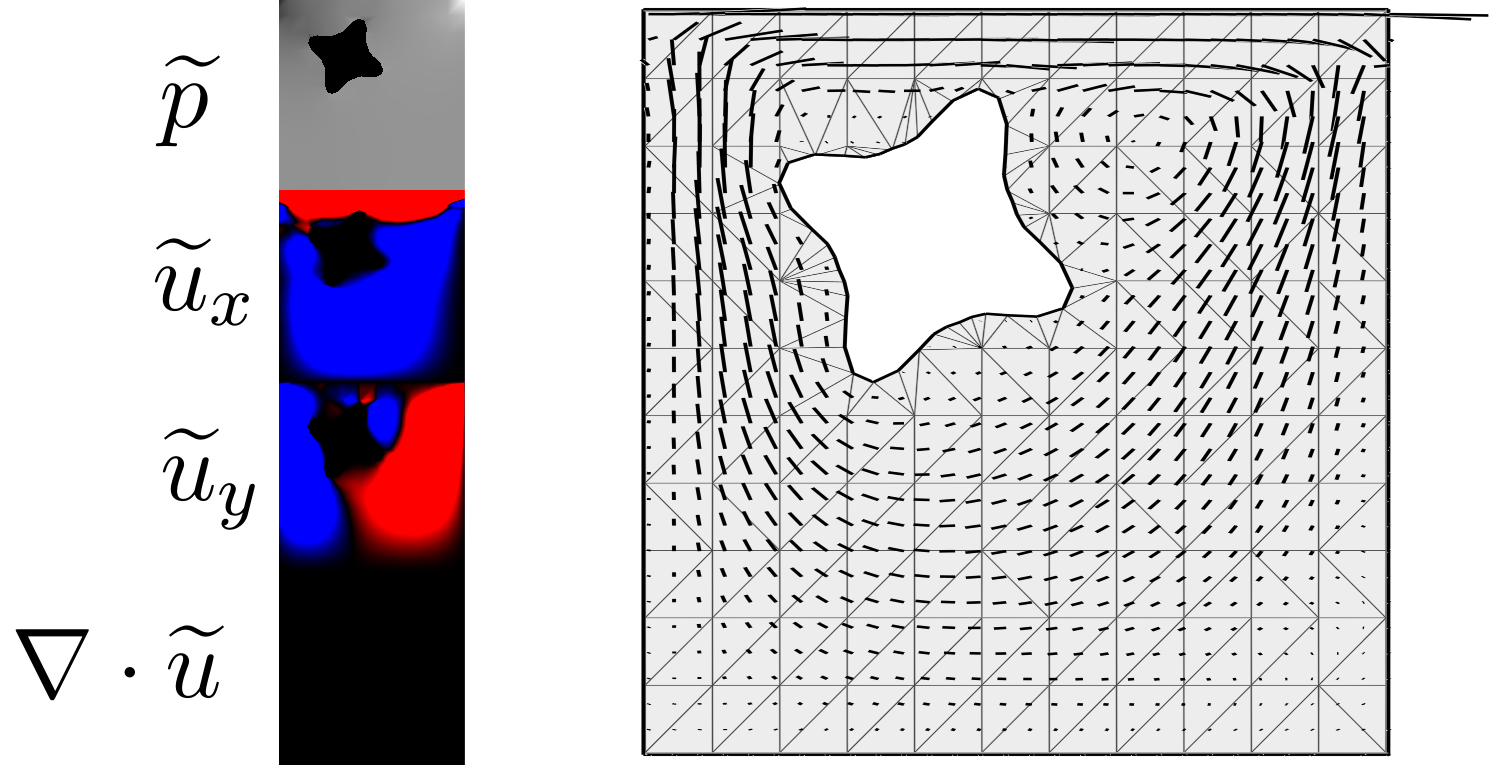
\includegraphics[width=0.8\textwidth]{figures/stokes/lid_driven_obstruction/figure.png}}
    \label{stokes_lid_driven_obstruction}
\end{figure}


% \begin{align*}
%     &\widetilde{u}_x\\
%     &\widetilde{u}_y\\
%     &\widetilde{p}\\
%     &\nabla\cdot \widetilde{u}
% \end{align*}
% 
% After one iteration.
% 
% After about 20 iterations.
% 
% After about 100 iterations.
